\section{Evaluation} \label{sec:evaluation}

\cnote{C27}{Whole section: the analysis prose after Table~1 (six paragraphs) is long and thin. Replace it by (i)~a small table with completed/timed-out queries per system and semantics and the $n$ of each column group, (ii)~two or three paragraphs that state facts with numbers, (iii)~a per-query YAGO-2S table. Net length about the same, but it answers ADBIS D1/D3/D5 and review-ai.md, M4.}
We evaluate the proposed solution (LARPQ) on three semantics (all-simple-paths, all-shortest-paths, and all-trails) using real-world knowledge graphs.
The experiments are designed to answer the following research questions.

\begin{itemize}
    \item \textbf{RQ1:} How does our implementation compare with production graph database systems?
    \item \textbf{RQ2:} What is the performance behavior across different query types and graph structures?
\end{itemize}

Experiments are conducted on a workstation equipped with a Ryzen 9 7900X (4.7 GHz, 12 cores), 128 GB of DDR5 RAM, running Ubuntu 22.04.
The timeout is set to 60 seconds per query.
Each query is executed five times: one warm-up run followed by four measurement runs.

\paragraph{Competitors.}
% C28 (2026-09-17): \subsubsection without \subsection rendered as 6.0.1.
%\subsubsection{Competitors}

We compare the performance of the proposed semiring-based LARPQ algorithm against state-of-the-art graph database management systems.
\begin{itemize}
    \item \textbf{MillenniumDB} or MDB (RPQ challenge version)~\cite{millenniumdb}: a persistent, open-source graph database with state-of-the-art RPQ performance and natural support of all three path semantics. 
    \item \textbf{FalkorDB} (v4.18.5, formerly RedisGraph~\cite{redisgraph}): an open-source in-memory property-graph database using GraphBLAS. Among the three path semantics, only all-trails is naturally expressed in FalkorDB, so we measure only the corresponding queries.
\end{itemize}

For all competitors, we use their respective query languages to specify queries.
The time required for query processing (including parsing and optimization) is included in the measurements.
All data is preloaded into storage, so graph preprocessing time is excluded from the results.

\paragraph{Datasets.}
%\subsubsection{Dataset}

We used three different graphs and their respective sets of queries.

\textbf{Wikidata~\cite{wikidata}}: $610$ million edges, $91$ million vertices, and $1\,400$ distinct labels. A total of $578$ queries were filtered from a dump of $660$ queries.

\textbf{Yago-2S}: $46$ million edges, $7$ million vertices, and $42$ distinct labels. Seven complex queries were taken from \cite{yago-queries}.

\textbf{RPQBench~\cite{rpqbench}}: a synthetic dataset with $150$ million edges, $57$ million vertices, and $9$ distinct labels. It includes $20$ different query types, $10$ queries were generated for each.

\subsection{Experimental Results}

We measure the total time for all queries, the mean and median time over all queries, and the mean and median per-query speedup over the proposed solution.
A summary for all three graphs is presented in Table~\ref{tab:results}.
Per-query results for Wikidata are shown in Figure~\ref{fig:wikidata_results}. 
Only queries that were successfully evaluated for all competitors are included in these statistics.
Figure~\ref{fig:wikidata_trails_wo_falkordb} additionally shows queries completed by MillenniumDB and our solution but not by FalkorDB.

\begin{table*}[t]
	\centering
	\caption{Performance summary on Wikidata, RPQBench, and YAGO-2S (time in milliseconds). For YAGO-2S under the simple-paths and trails semantics only two of seven queries completed on all systems, so only total time is reported; FalkorDB timed out on all YAGO-2S queries (---).}
	\label{tab:results}
	\begin{tabular}{|l|l|c c|c c|c c c|}
		\hline
		\multirow{2}{*}{Dataset} & \multirow{2}{*}{Metric} & \multicolumn{2}{|c|}{Simple} & \multicolumn{2}{|c|}{Shortest} & \multicolumn{3}{|c|}{Trails} \\
		 & & \textbf{LARPQ} & \textbf{MDB} & \textbf{LARPQ} & \textbf{MDB} & \textbf{LARPQ} & \textbf{MDB} & \textbf{FalkorDB} \\
		\hline
		\hline
		\multirow{5}{*}{Wikidata}
		& Total time     & \textbf{224\,682} & 1\,111\,429 & \textbf{205\,629} & 780\,011 & 152\,128     & 921\,506 & \textbf{81\,519} \\
		& Mean time      & \textbf{428}      & 2\,121      & \textbf{392}      & 1\,488   & 312          & 1\,892   & \textbf{167}     \\
		& Median time    & \textbf{1.7}      & 36.6        & \textbf{2.0}      & 27.9     & \textbf{1.4} & 36.9     & 4.5              \\
		& Mean speedup   & \textbf{1.0}      & 0.6         & \textbf{1.0}      & 0.8      & \textbf{1.0} & 0.5      & 0.9              \\
		& Median speedup & \textbf{1.0}      & 0.1         & \textbf{1.0}      & 0.1      & \textbf{1.0} & 0.1      & 0.7              \\
		\hline
		\multirow{5}{*}{RPQBench}
		& Total time     & \textbf{857} & 2\,836       & \textbf{890} & 3\,253       & \textbf{849} & 3\,256       & 1\,685       \\
		& Mean time      & \textbf{43}  & 142          & \textbf{45}  & 162          & \textbf{53}  & 203          & 105          \\
		& Median time    & 0.3          & \textbf{0.2} & 0.3          & \textbf{0.1} & 0.3          & \textbf{0.2} & \textbf{0.2} \\
		& Mean speedup   & 1.0          & \textbf{1.5} & 1.0          & \textbf{2.1} & 1.0          & \textbf{1.5} & 1.2          \\
		& Median speedup & 1.0          & \textbf{1.8} & 1.0          & \textbf{2.4} & 1.0          & \textbf{1.7} & 1.5          \\
		\hline
		\multirow{5}{*}{YAGO-2S}
		& Total time     & \textbf{105} & 215 & \textbf{1\,195} & 1\,956 & \textbf{66} & 479 & --- \\
		& Mean time      & ---          & --- & \textbf{171}    & 279    & ---         & --- & --- \\
		& Median time    & ---          & --- & \textbf{167}    & 268    & ---         & --- & --- \\
		& Mean speedup   & ---          & --- & \textbf{1.0}    & 0.5    & ---         & --- & --- \\
		& Median speedup & ---          & --- & \textbf{1.0}    & 0.6    & ---         & --- & --- \\
		\hline
	\end{tabular}
\end{table*}

\cnote{C29}{Generic; cut. The informal simple/hard definition in the next sentence should go too (use ``above/below the median'' or a threshold). About 3 lines.}
The evaluation shows that execution time strongly depends on the particular query and the choice of start and target vertices.
We define a query as \emph{simple} for a system if it requires relatively little time to evaluate, and \emph{hard} if, conversely, it requires a relatively large amount of time.

For RPQBench (Table~\ref{tab:results}), the total and mean execution times of our solution are more than three times better than those of the competitors across all semantics. However, the median time and per‑query speedup favor the competitors. This indicates that the dataset contains a relatively large number of simple queries, while our solution exhibits a significant advantage on harder queries.

\cnote{C30}{Also inaccurate for Wikidata, where LARPQ wins the median as well (1.7 vs 36.6~ms). Merge this and the next two sentences into one paragraph on the shape of the distributions. About 2 lines.}
This observation is consistent with the results presented in Figure~\ref{fig:wikidata_results}, where MillenniumDB outperforms our solution on simple queries but is slower on hard ones. 
The tail of queries that are challenging for all solutions is thinner for LARPQ than for MillenniumDB and FalkorDB, as illustrated in Figure~\ref{fig:wikidata_trails_common}.
Additionally, we observe that in the common-trails setting, FalkorDB achieves the best total and mean times, while LARPQ achieves the best median time, which is also consistent with the shape of the hard queries tail.

\cnote{C31}{Four sentences for two numbers. With a per-query YAGO-2S table (7 rows $\times$ 3 semantics) this is one sentence, and the ``---'' cells in Table~1 can go. About 3 lines.}
Analysis of the YAGO-2S dataset (see Table~\ref{tab:results}) shows that the shortest‑path semantics is the only one for which all seven queries completed successfully across all competing systems.
For the simple‑paths and trails semantics, only two of the seven queries were completed by all systems within the 60-second timeout; the remaining queries timed out on every solution, and FalkorDB timed out on all YAGO-2S queries.
Therefore, for these two semantics, Table~\ref{tab:results} reports only the total time over the two completed queries and omits the mean, median, and speedup, which are not meaningful for such a small sample.
For the queries that did complete, our solution is faster than the competitors, but this observation is based on two queries only.

\cnote{C32}{Unsupported here (no per-type data is shown): either add a per-type RPQBench figure, which would also answer RQ2, or reduce to one sentence citing [6]. The ``Overall, \ldots'' sentence below repeats it; keep one of the two. About 4 lines.}
A detailed analysis of which queries are \emph{simple} and which are \emph{hard} for our solution yields results similar to those reported in~\cite{belyanin2150single}, indicating that the proposed generalization significantly inherits the properties of the basic version. Specifically, LARPQ outperforms competitors on queries with complex patterns over labels corresponding to many edges (e.g., $l_1 \cdot l_2 \cdot (l_3 \mid l_4)^*$), while on queries with simple patterns such as $l_1^* \cdot  l_2$, it shows no performance advantage, and MillenniumDB may be a better choice.

Overall, the results indicate that LARPQ is a strong choice for complex RPQs, especially when query patterns involve labels with many matching edges, whereas competing systems may perform better on simpler patterns.

\cnote{C33}{Fig.~3 takes about 0.4 page for four panels whose tick labels are unreadable. One panel with grouped violins (system $\times$ semantics) on a shared log axis, or a CDF of per-query time ratios, is smaller and directly comparable. About 0.2 page.}
\begin{figure*}[t]
\centering
\begin{subfigure}[t]{0.24\textwidth}
        \centering
        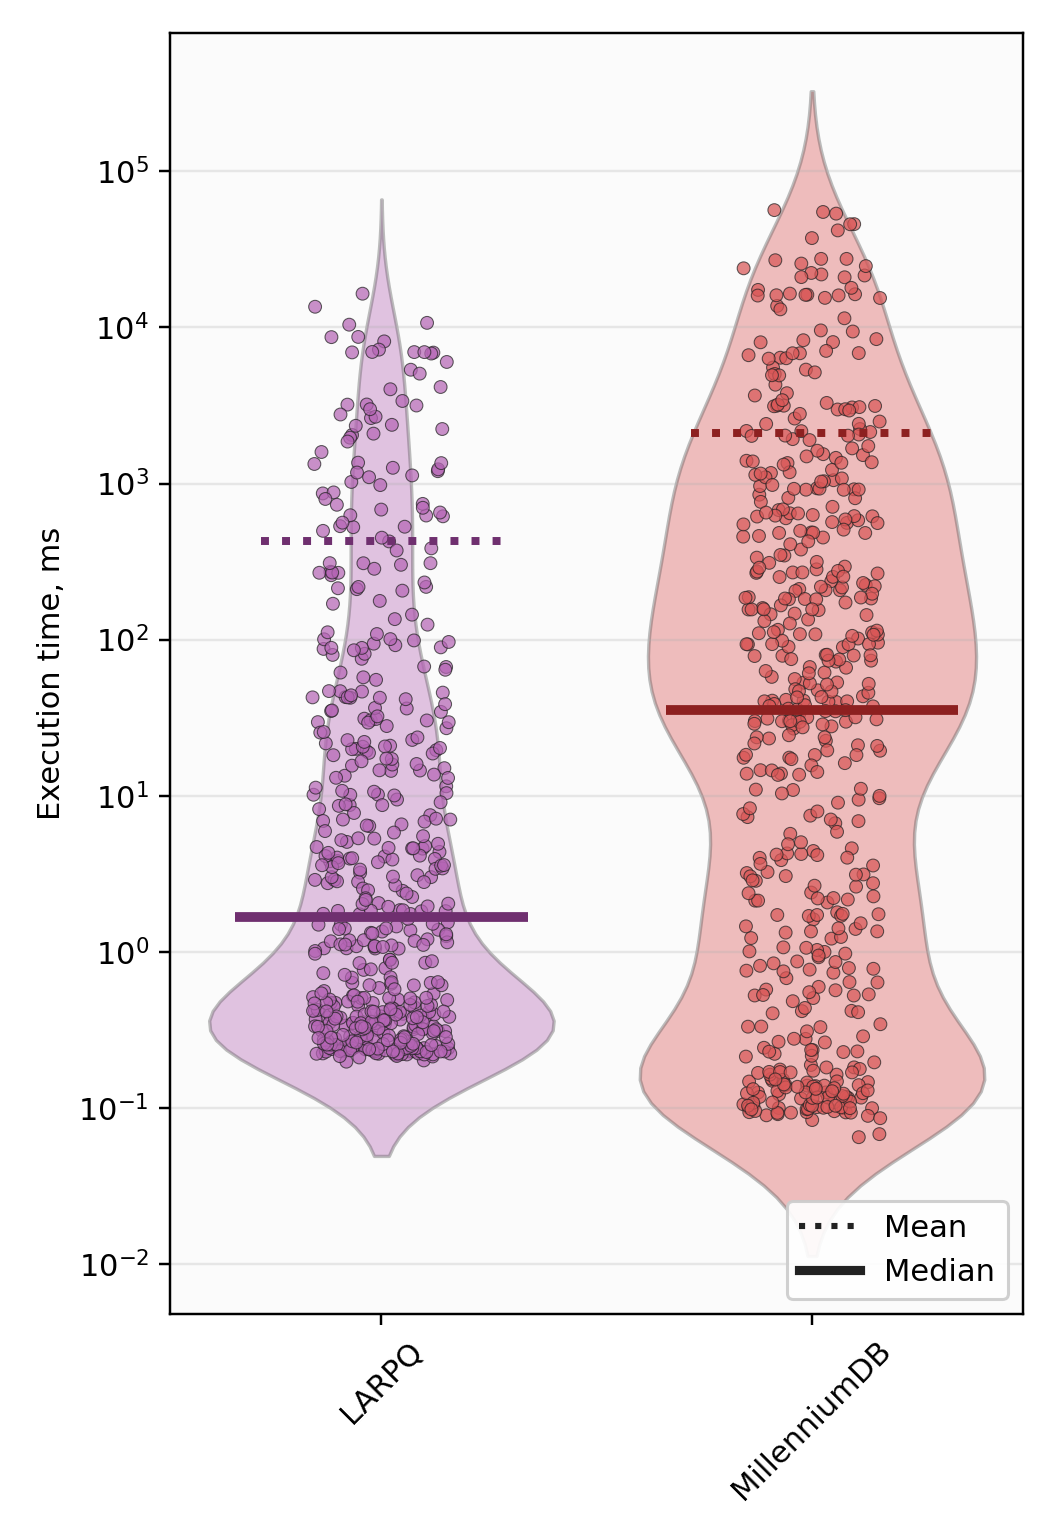
\includegraphics[width=\linewidth]{figures/wikidata_simple_common_violin.png}
		\caption{Simple paths}
        \label{fig:wikidata_simple}
    \end{subfigure}
    \hfill
    \begin{subfigure}[t]{0.24\textwidth}
        \centering
        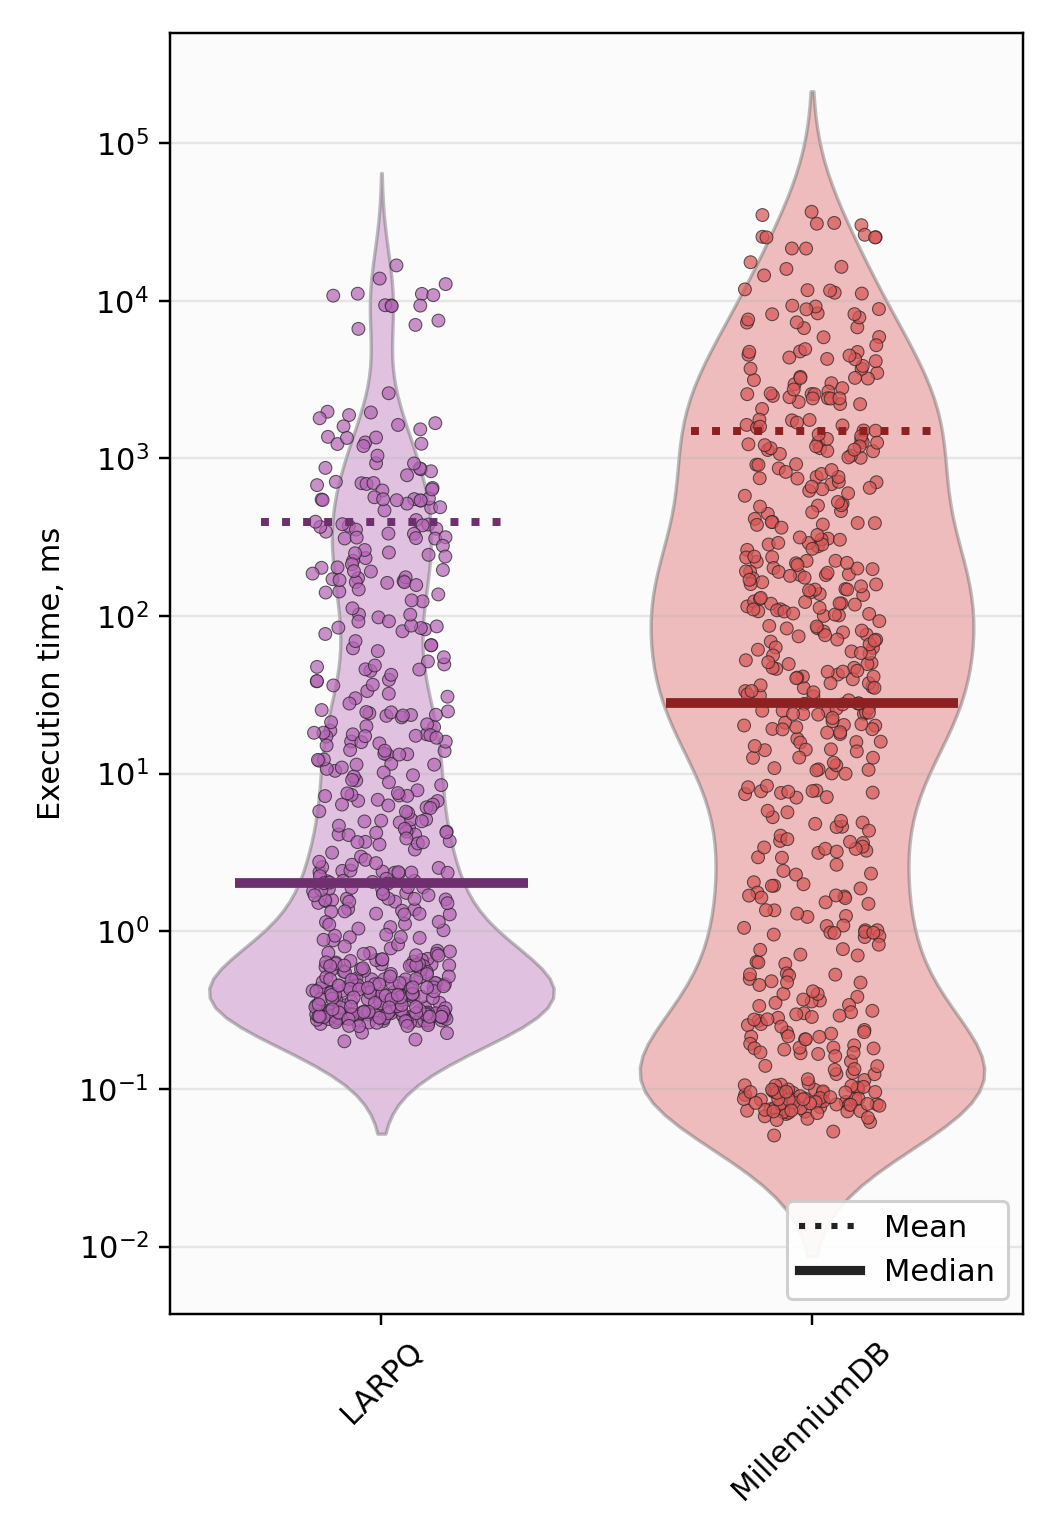
\includegraphics[width=\linewidth]{figures/wikidata_all_shortest_common_violin.png}
        \caption{Shortest paths}
        \label{fig:wikidata_shortest}
    \end{subfigure}
	\begin{subfigure}[t]{0.24\textwidth}
        \centering
        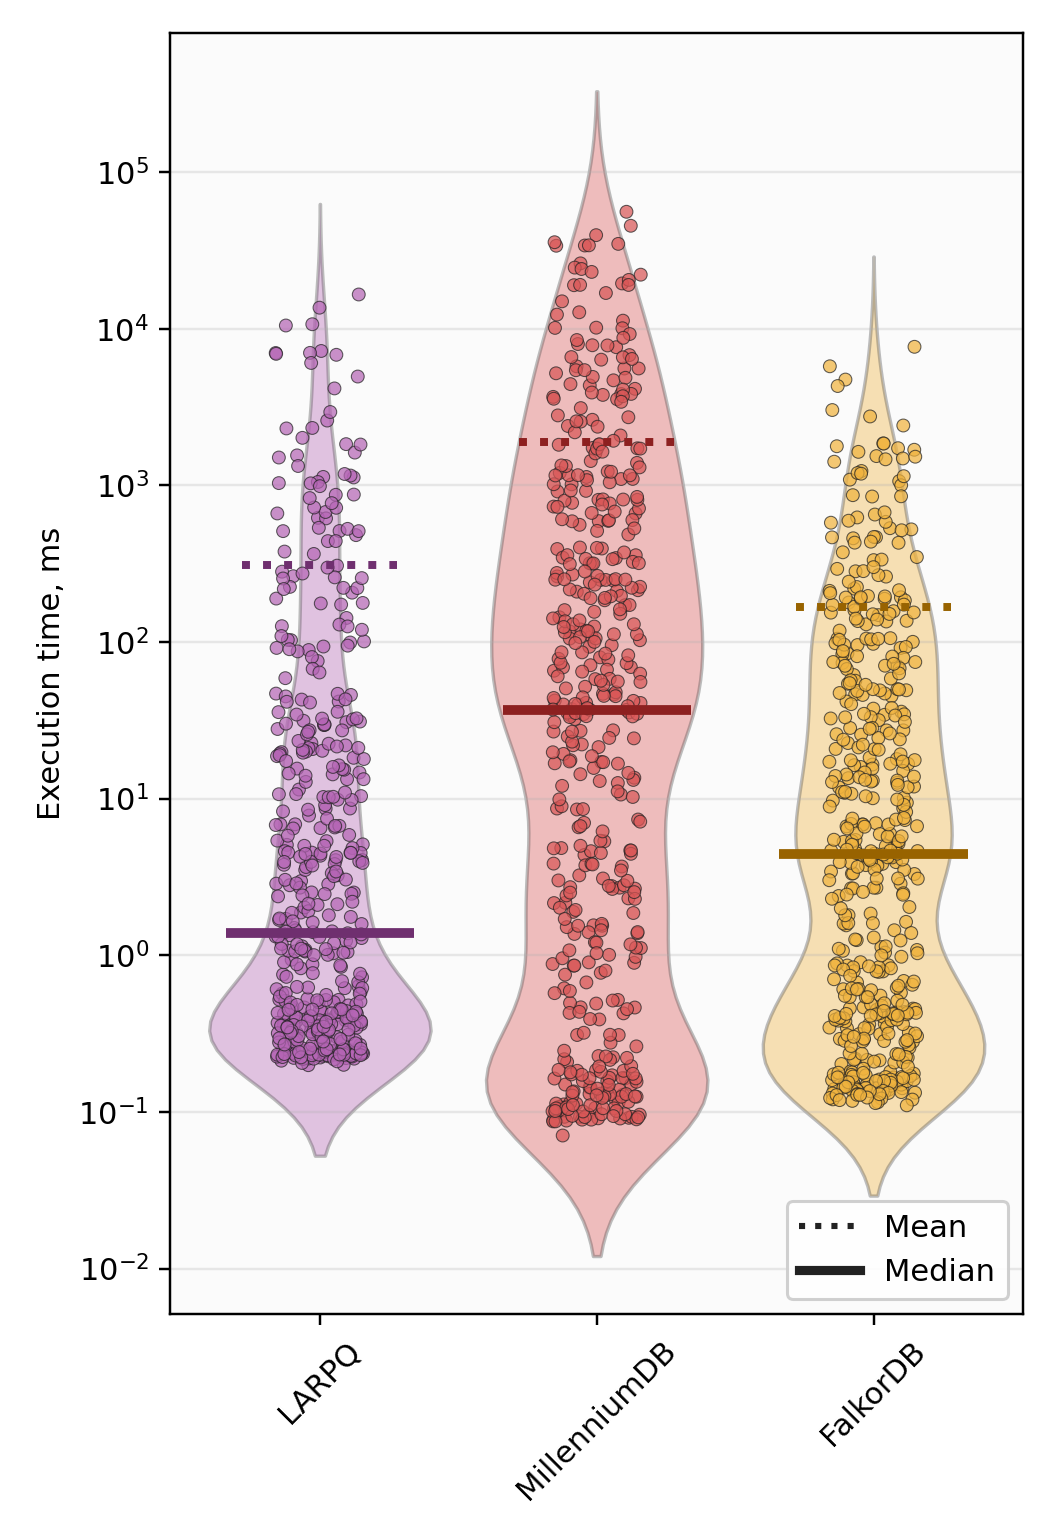
\includegraphics[width=\linewidth]{figures/wikidata_trails_common_violin.png}
        \caption{Trails (common for all competitors)}
        \label{fig:wikidata_trails_common}
    \end{subfigure}
    \hfill
    \begin{subfigure}[t]{0.24\textwidth}
        \centering
        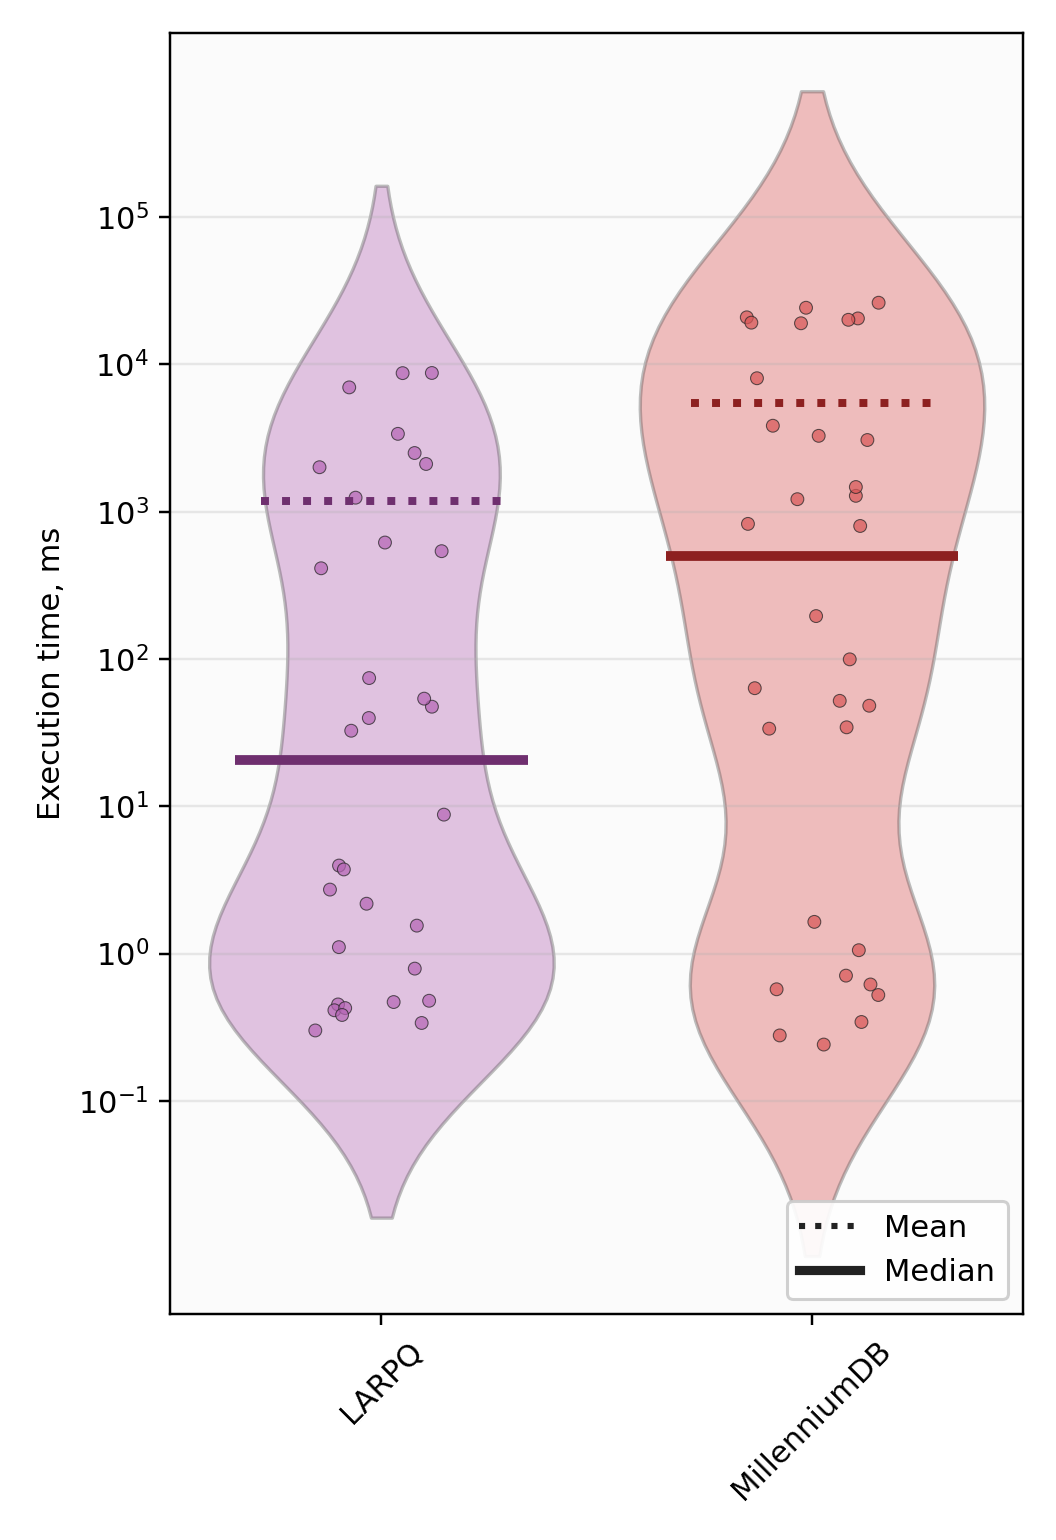
\includegraphics[width=\linewidth]{figures/wikidata_trails_falkor_failed_violin.png}
        \caption{Trails (FalkorDB failed)}
        \label{fig:wikidata_trails_wo_falkordb}
    \end{subfigure}
\caption{Per-query execution time on Wikidata (log scale). Each point is one query; solid and dotted lines are the median and the mean.}
\label{fig:wikidata_results}
\end{figure*}

